\begin{figure}[t]
  \centering
  \begin{minipage}[t]{\textwidth}
    % Left-side labels
    \begin{minipage}[t]{0.045\textwidth}
      \footnotesize\raggedleft
      \vspace{-2.75cm} % align with top of images
      SIMSE\\[0.4cm]
      L1\\[0.385cm]
      JTFS\\[0.365cm]
      DTW
    \end{minipage}%
    \hspace{0.01\textwidth}%
    % Right side: images + captions
    \begin{minipage}[t]{0.91\textwidth}
      \centering
      \begin{minipage}[t]{0.31\textwidth}
        \centering
        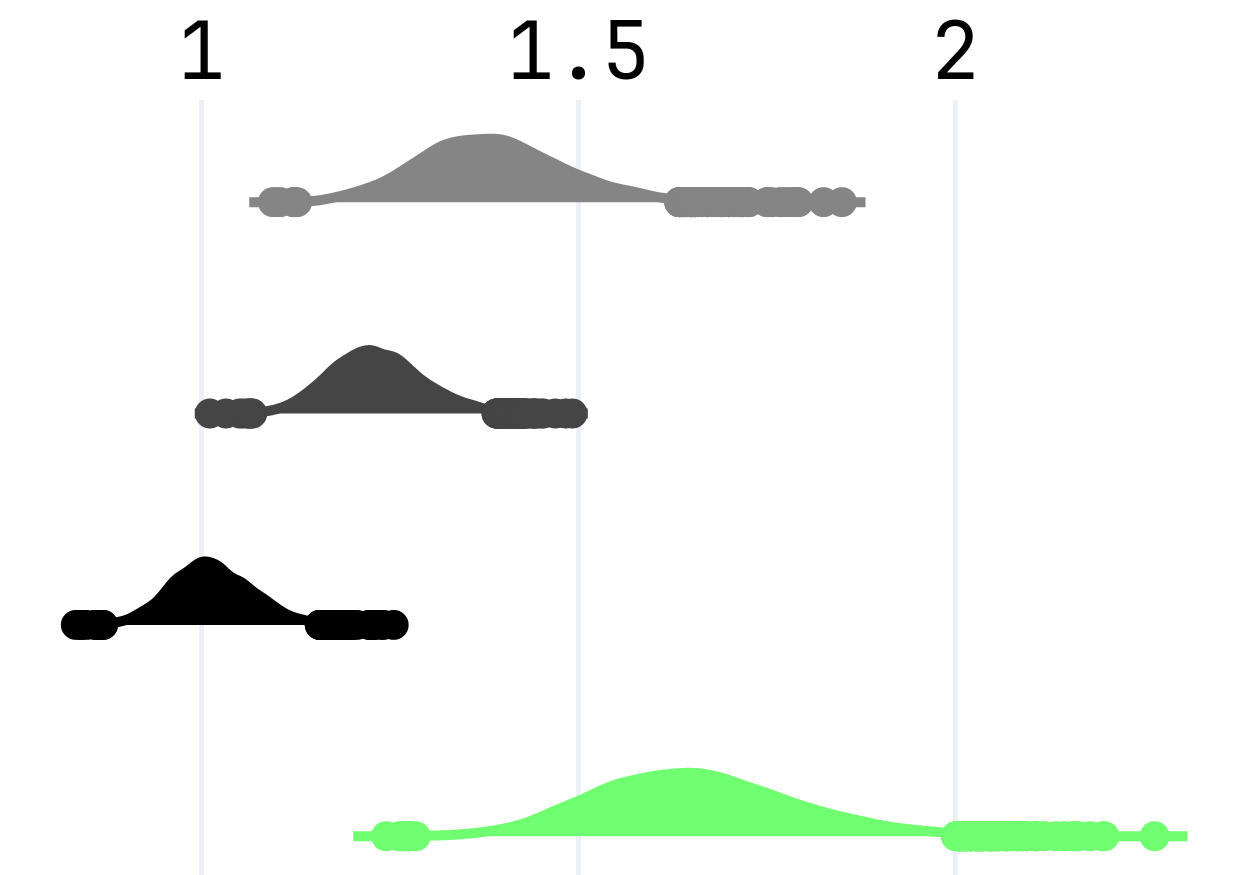
\includegraphics[width=\linewidth]{images/npsk_ood_P_Loss_0.png}
        \vspace{0.3em}
        \footnotesize Non-Overlapping Frequencies
      \end{minipage}
      \hspace{0.015\textwidth}%
      \begin{minipage}[t]{0.31\textwidth}
        \centering
        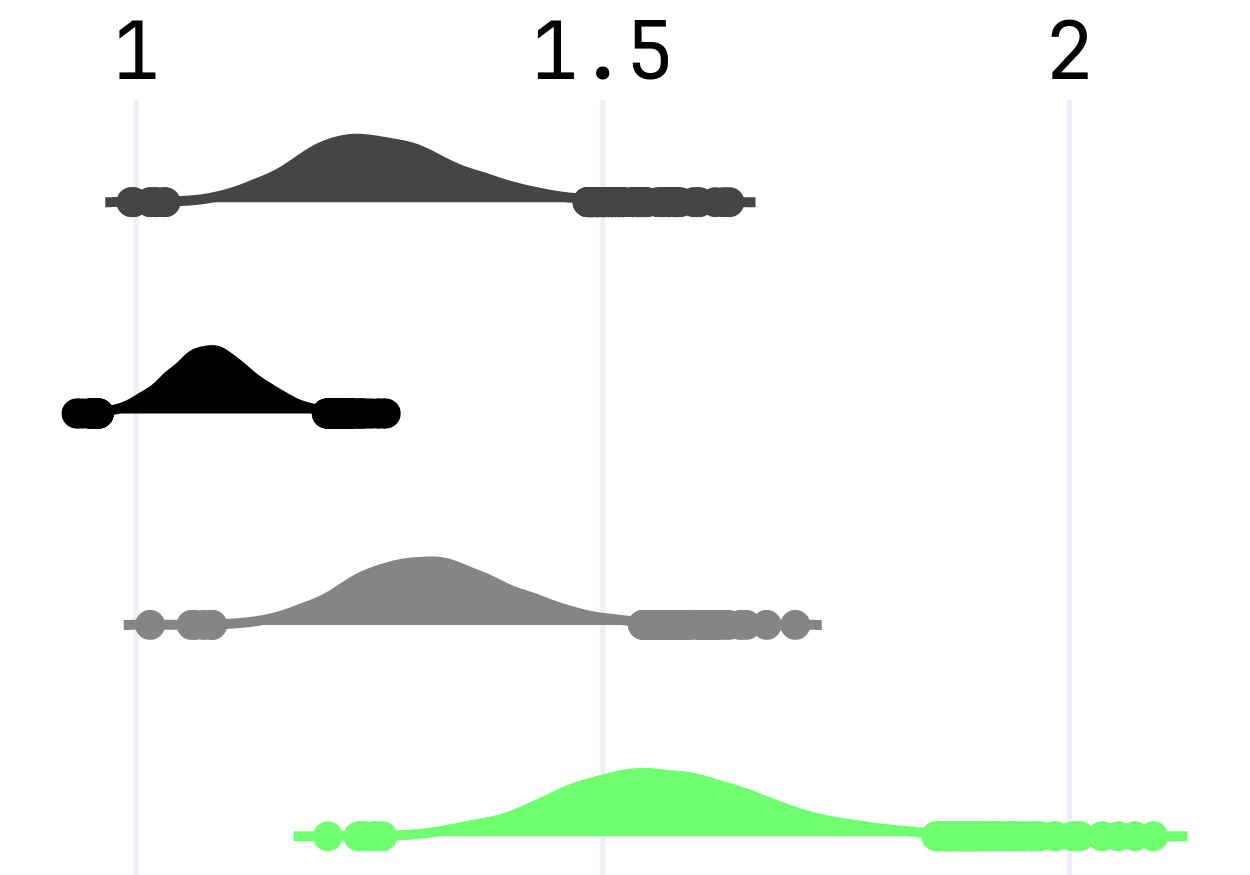
\includegraphics[width=\linewidth]{images/npsk_ood_P_Loss_1.png}
        \vspace{0.3em}
        \footnotesize Sine Target, Saw Imitator
      \end{minipage}
      \hspace{0.01\textwidth}%
      \begin{minipage}[t]{0.31\textwidth}
        \centering
        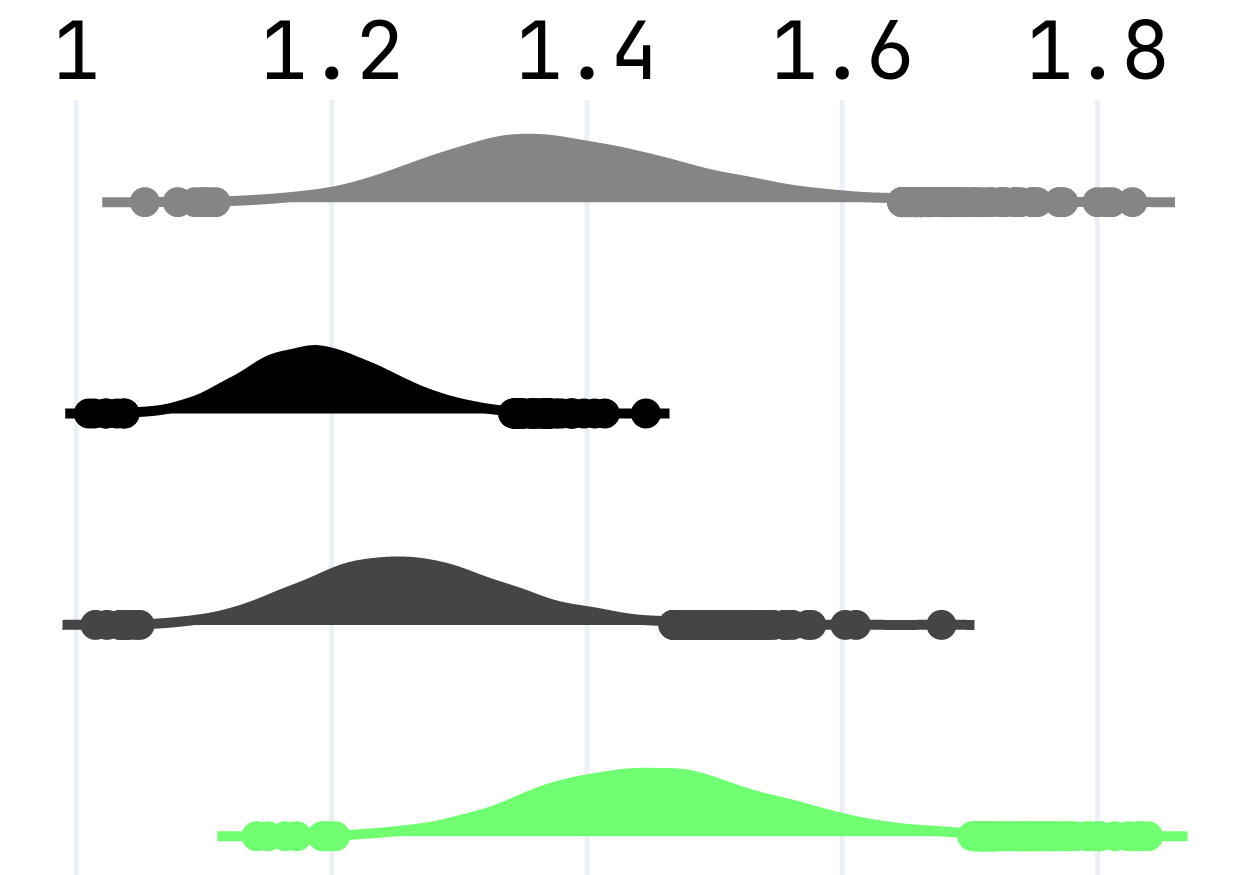
\includegraphics[width=\linewidth]{images/npsk_ood_P_Loss_2.png}
        \vspace{0.3em}
        \footnotesize Saw Target, Sine Imitator
      \end{minipage}
    \end{minipage}
  \end{minipage}
  \caption{Bootstrapped distributions and ranks for AM-Synthesizer sound matching.}
  \label{fig:npsk_am_synths}
\end{figure}